% Provenance (never printed): lycee terminale S SVT "Les climats de la Terre"
% and the 2019 enseignement scientifique ("Le climat de la Terre": forcing,
% feedbacks, the IPCC assessments, scenarios), union; physical science only,
% as the user ruled (2026-10-22). See sources/outline_sources.md. Pilot
% chapter, 2026-10-22. Every figure about the climate system is an IPCC AR6
% WG1 statement (ledger ipcc:*) or computed from a dataset in
% figdata/grade-12/climate_records.py.
\chapter{تغير المناخ: الأرصاد والأسباب والإسقاطات}\label{ch:g12:climate-change}

عاليًا على المنحدر الشمالي لماونا لوا، وهو بركان في وسط
المحيط الهادئ، تقف مجموعة من المباني البيضاء على لابة عارية،
على ارتفاع \qty{3397}{m} فوق البحر. وهناك، فوق طبقة الهواء التي تلوثها
الجزيرة في الأسفل، وعلى بعد آلاف الكيلومترات من أي مدينة كبيرة، يكون الهواء
نقيًّا وممتزجًا جيدًا تقريبًا كالغلاف الجوي للكوكب كله. ومنذ
مارس 1958، يُقاس ما فيه من ثاني أكسيد الكربون دون انقطاع تقريبًا.
بدأ السجل مشروعًا لكيميائي واحد؛ ثم صار أشهر
منحنى في علوم الأرض. يقرأ هذا الفصل ذلك المنحنى وسائر سجلات
المناخ، ويشرح كيف يغيّر تغيرٌ في الهواء \omterm{def:g10:earth-energy-budget:energy-budget}{ميزانية الطاقة}
للكوكب، وكيف يقرر العلماء ما الذي سبّب الاحترار الذي يرصدونه،
وما الذي يتوقعونه في إسقاطاتهم للعقود القادمة.
% ledger: noaa:mlo-site, noaa:keeling-1958

\begin{omfigure}
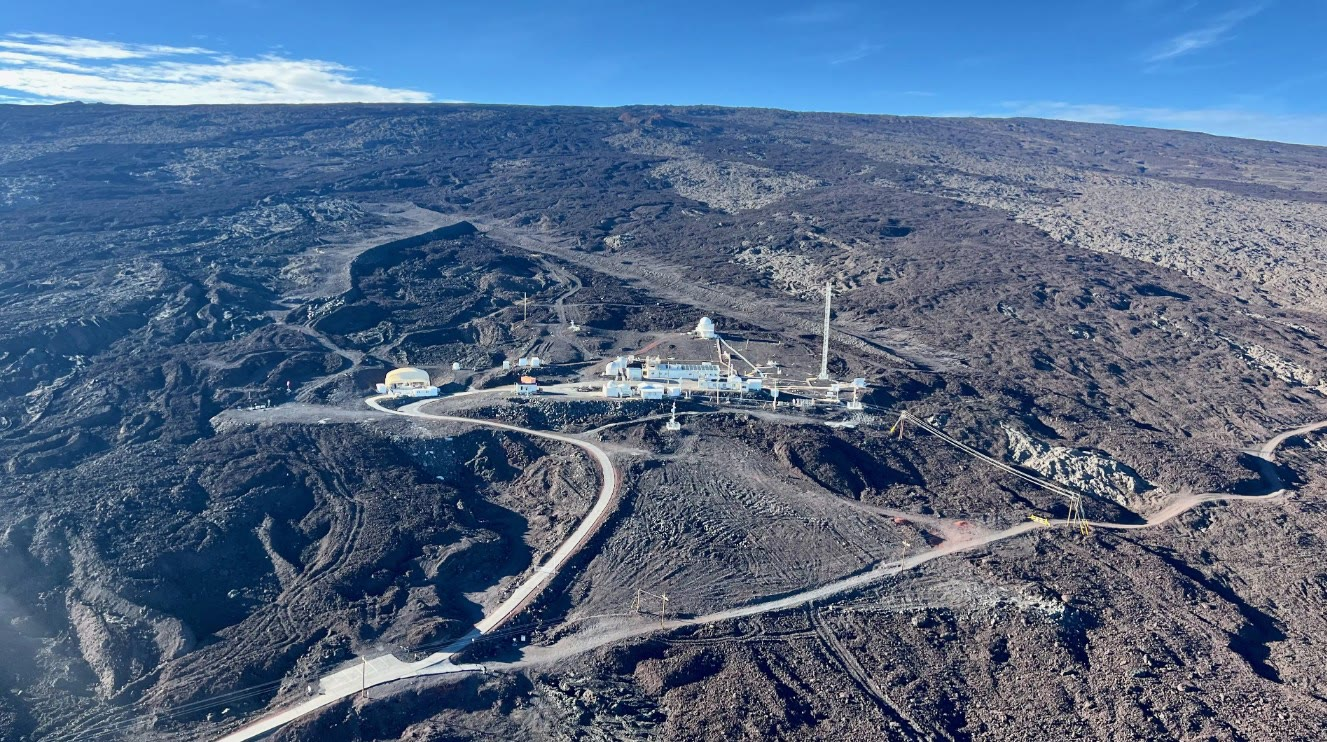
\includegraphics[width=0.78\linewidth]{images/book2/g12-noaa-mauna-loa-observatory.jpg}

{\small مرصد ماونا لوا، هاواي، على مسيلات لابية قديمة عاليًا على
الجانب الشمالي للبركان. الصورة: براين فاسل، الإدارة الوطنية للمحيطات والغلاف الجوي الأمريكية (ملك عام).}
\end{omfigure}

\begin{recall}
تتلقى الأرض طاقة من الشمس على هيئة ضوء، وتفقد المقدار نفسه في
المتوسط إلى الفضاء على هيئة أشعة تحت حمراء؛ وحصة ضوء الشمس المنعكسة
هي \omterm{def:g10:earth-energy-budget:albedo}{الألبيدو} (\cref{ch:g10:earth-energy-budget}). وغازات الدفيئة --- بخار
الماء، وثاني أكسيد الكربون، والميثان --- تمتص جزءًا من الأشعة تحت الحمراء التي يطلقها
السطح وتعيد جزءًا منها إلى الأسفل؛ وأثر الدفيئة هذا يُبقي
السطح أدفأ بكثير مما كان سيكون بدونه (كتب الكيمياء،
والكتاب 1، الصف 9). وتحفظ \omterm{def:g12:past-climates:ice-core}{العينات الجليدية} فقاعات من الهواء القديم وتسجل
\omterm{def:g12:past-climates:glacial-cycle}{الدورات الجليدية} على مدى \num{800000} السنة الأخيرة (\cref{ch:g12:past-climates}).
\end{recall}

\section{السجلات}

\begin{omfigure}
\begin{tikzpicture}
\begin{axis}[omrecord, width=0.92\linewidth, height=6.2cm, xmin=1957, xmax=2028,
  ymin=305, ymax=440, xlabel={السنة}, ylabel={\foreignlanguage{arabic}{ثاني أكسيد الكربون \babelsublr{(ppm)}}},
  xtick={1960,1970,...,2020}, /pgf/number format/1000 sep={}]
\addplot[omDef!85!black, line width=0.5pt] table[x=decimal_year, y=co2_ppm] {figdata/out/grade-12-climate_records-co2.dat};
\addplot[only marks, mark=*, mark size=0.9pt, omThm!85!black] table[x=year, y=co2_ppm] {figdata/out/grade-12-climate_records-co2annual.dat};
\end{axis}
\end{tikzpicture}

{\small محتوى الهواء من ثاني أكسيد الكربون في ماونا لوا: المتوسطات الشهرية
(الخط) والمتوسطات السنوية (النقاط)، بأجزاء من المليون (ppm) من الهواء الجاف.
البيانات: مختبر الرصد العالمي التابع للإدارة الوطنية للمحيطات والغلاف الجوي الأمريكية، ومعهد سكريبس لعلوم
المحيطات.}
\end{omfigure}

\begin{proposition}[سجل ثاني أكسيد الكربون]\label{prop:g12:climate-change:co2}
% ledger: data:co2-mlo (all numbers computed in figdata/grade-12/climate_records.py)
في ماونا لوا، ارتفع المتوسط السنوي لتركيز ثاني أكسيد الكربون من
\qty{316.0}{ppm} عام 1959 إلى \qty{427.4}{ppm} عام 2025، والارتفاع
يتسارع: فقد زاد التركيز بنحو \qty{0.9}{ppm} في السنة في
ستينيات القرن العشرين، وبنحو \qty{2.6}{ppm} في السنة بين 2015 و2025. وفي كل
سنة يتأرجح التركيز أيضًا بنحو \qty{7}{ppm}: فهو أعلى ما يكون في
مايو وأدنى ما يكون في سبتمبر.
\end{proposition}

\begin{remark}[لماذا للمنحنى أسنان]\label{rem:g12:climate-change:teeth}
التأرجح السنوي هو تنفّس الغطاء النباتي في نصف الكرة
الشمالي، حيث توجد معظم نباتات اليابسة. ففي الربيع والصيف، تأخذ النباتات
من ثاني أكسيد الكربون بالتمثيل الضوئي أكثر مما تطلقه هي والتربة؛
وفي الخريف والشتاء، تغلب التحلل والتنفس. أما الارتفاع من سنة إلى
سنة فقصة أخرى: إنه كربون الوقود الأحفوري والغابات
المزالة يتراكم في الهواء.
\end{remark}

\begin{proposition}[أعلى مما كان منذ مليوني سنة على الأقل]\label{prop:g12:climate-change:icecore}
% ledger: data:co2-bereiter (173.7 and 298.6 ppm computed), ipcc:co2-2myr (high confidence)
على مدى \num{800000} السنة الأخيرة، تسجل فقاعات الهواء في جليد القارة القطبية الجنوبية
تراكيز لثاني أكسيد الكربون بين نحو \qty{174}{ppm}، في أبرد
\omterm{def:g12:past-climates:glacial-cycle}{الفترات الجليدية}، و\qty{299}{ppm}، في أدفأ \omterm{def:g12:past-climates:glacial-cycle}{الفترات بين الجليدية}. وقيمة اليوم
تزيد بأكثر من \qty{100}{ppm} على أعلاها.
وتقرر التقييمات أن التركيز في عام 2019 كان أعلى منه في أي وقت
خلال مليوني سنة على الأقل (\emph{بثقة عالية}).
\end{proposition}

\begin{omfigure}
\begin{tikzpicture}
\begin{axis}[omrecord, omage, width=0.92\linewidth, height=5.2cm, xmin=0, xmax=810,
  ymin=150, ymax=490, xlabel={\foreignlanguage{arabic}{آلاف السنين قبل عام 1950}},
  ylabel={\foreignlanguage{arabic}{ثاني أكسيد الكربون \babelsublr{(ppm)}}}, xtick={0,100,...,800}]
\addplot[omDef!85!black, line width=0.6pt] table[x=age_kyr, y=co2_ppm] {figdata/out/grade-12-climate_records-icecore.dat};
\draw[omThm, densely dashed, line width=0.8pt] (axis cs:810,427.35) -- (axis cs:0,427.35);
\node[font=\footnotesize, text=omThm!85!black, anchor=south west] at (axis cs:780,433) {\foreignlanguage{arabic}{المتوسط السنوي في ماونا لوا عام 2025}};
\end{axis}
\end{tikzpicture}

{\small ثاني أكسيد الكربون في جليد القارة القطبية الجنوبية على مدى \num{800000} سنة: تحرّكه \omterm{def:g12:past-climates:glacial-cycle}{الدورات
الجليدية} بين نحو 180 و\qty{300}{ppm}. والذروة الدقيقة عند الطرف
الأيمن هي أحدث الجليد، الذي يسجل بداية الارتفاع الحالي،
حتى عام 2001. البيانات: بيرايتر وآخرون (2015)، قسم المناخ القديم في
الإدارة الوطنية للمحيطات والغلاف الجوي الأمريكية.}
% the youngest sample of the composite: age -51 yr BP (2001), 368.02 ppm (data/derived/co2-icecore.csv)
\end{omfigure}

\begin{omfigure}
\begin{tikzpicture}
\begin{axis}[omrecord, width=0.92\linewidth, height=5.6cm, xmin=1878, xmax=2027,
  ymin=-0.6, ymax=1.45, xlabel={السنة},
  ylabel={\foreignlanguage{arabic}{شذوذ درجة الحرارة \babelsublr{(\unit{\degreeCelsius})}}},
  xtick={1880,1900,...,2020}, /pgf/number format/1000 sep={},
  legend style={at={(0.03,0.96)}, anchor=north west, font=\footnotesize, draw=black!30}]
\addplot[omDef!70, line width=0.5pt, mark=*, mark size=0.6pt] table[x=year, y=anomaly] {figdata/out/grade-12-climate_records-temp.dat};
\addlegendentry{المتوسط السنوي}
\addplot[omThm!85!black, line width=1.3pt, unbounded coords=jump] table[x=year, y=mean11] {figdata/out/grade-12-climate_records-temp.dat};
\addlegendentry{\foreignlanguage{arabic}{المتوسط على 11 سنة}}
\end{axis}
\end{tikzpicture}

{\small متوسط درجة الحرارة العالمية عند السطح، بوصفه الفرق عن متوسطها
في 1951--1980. البيانات: تحليل درجة حرارة السطح لمعهد غودارد لدراسات الفضاء التابع لناسا (GISTEMP، الإصدار~4).}
\end{omfigure}

\begin{proposition}[الاحترار العالمي المرصود]\label{prop:g12:climate-change:warming}
% ledger: ipcc:gsat-2011-2020, ipcc:decades
كان كل عقد من العقود الأربعة الأخيرة أدفأ من أي عقد سبقه
منذ 1850. وكانت درجة الحرارة العالمية عند السطح في 2011--2020 أعلى بمقدار \qty{1.09}{\degreeCelsius}
مما كانت في 1850--1900 (على نحو مرجح جدًا بين 0.95
و\qty{1.20}{\degreeCelsius})، مع احترار أكبر فوق اليابسة
(\qty{1.59}{\degreeCelsius}) منه فوق المحيط (\qty{0.88}{\degreeCelsius}).
\end{proposition}

\begin{proposition}[البحر يرتفع أسرع فأسرع]\label{prop:g12:climate-change:sea}
% ledger: ipcc:sea-level-obs, data:gmsl-lsa (3.2 mm/yr trend computed)
ارتفع المتوسط العالمي لمستوى سطح البحر بنحو \qty{0.20}{m} بين 1901 و2018.
وكان المعدل نحو \qty{1.3}{mm} في السنة من 1901 إلى 1971،
و\qty{1.9}{mm} في السنة من 1971 إلى 2006، و\qty{3.7}{mm} في السنة من
2006 إلى 2018 (\emph{بثقة عالية}). والأقمار الصناعية، التي تقيس ارتفاع
سطح البحر منذ 1993، تجد متوسطًا قدره \qty{3.2}{mm} في السنة على مدى
1993--2025. ويرتفع البحر لأن المحيط الذي يسخن يتمدد، ولأن
الأنهار الجليدية والأغطية الجليدية تفقد جليدًا يصب فيه.
\end{proposition}

\begin{omfigure}
\begin{tikzpicture}
\begin{axis}[omrecord, width=0.86\linewidth, height=5cm, xmin=1992, xmax=2026,
  ymin=-35, ymax=95, xlabel={السنة}, ylabel={\foreignlanguage{arabic}{مستوى سطح البحر \babelsublr{(mm)}}},
  /pgf/number format/1000 sep={}, xtick={1995,2000,...,2025}]
\addplot[omDef!85!black, line width=0.5pt] table[x=decimal_year, y=gmsl_mm] {figdata/out/grade-12-climate_records-sea.dat};
\end{axis}
\end{tikzpicture}

{\small المتوسط العالمي لمستوى سطح البحر مقيسًا من الفضاء، كل عشرة أيام تقريبًا
(بعد إزالة الإشارة الموسمية)، مقارنةً بصفر اعتباطي. بيانات قياس الارتفاع
مقدَّمة من مختبر قياس الارتفاع بالأقمار الصناعية التابع للإدارة الوطنية للمحيطات والغلاف الجوي الأمريكية.}
\end{omfigure}

\begin{dated}{2025}
% ledger: data:co2-mlo, data:gistemp (values read from the datasets as fetched 2026-10-22)
بلغ المتوسط السنوي لتركيز ثاني أكسيد الكربون في ماونا لوا عام 2025
\qty{427.35}{ppm}. وفي سجل ناسا لدرجة الحرارة، كانت أدفأ سنة حتى الآن
2024، بزيادة \qty{1.28}{\degreeCelsius} على متوسط 1951--1980.
\end{dated}

\section{التأثير الإشعاعي}

\begin{definition}[التأثير الإشعاعي]\label{def:g12:climate-change:forcing}
\emph{التأثير الإشعاعي}\index{تأثير إشعاعي} لتغيّر في
النظام المناخي --- مزيد من غازات الدفيئة، أو مزيد من جسيمات الهباء الجوي، أو شمس أشد سطوعًا ---
هو التغير الذي يحدثه في صافي تدفق الطاقة الداخل إلى
النظام المناخي عند قمة الغلاف الجوي، قبل أن تجد درجة حرارة السطح
وقتًا للاستجابة. ويُقاس بالواط لكل متر مربع
(\unit{W/m^2}) من سطح الأرض. فالتأثير الموجب يجعل الكوكب
يكسب طاقة ويسخن؛ والتأثير السالب يجعله يفقد طاقة ويبرد.
\end{definition}

\begin{remark}[التأثير الفعّال]\label{rem:g12:climate-change:effective}
تستعمل التقييمات \omterm{def:g12:climate-change:forcing}{التأثير الإشعاعي} \emph{الفعّال}، الذي يحسب أيضًا
التعديلات السريعة في الغلاف الجوي (في سحبه، مثلًا)
التي تحدث قبل أن يسخن السطح. وكل \omterm{def:g12:climate-change:forcing}{التأثيرات} في هذا الفصل
\omterm{def:g12:climate-change:forcing}{تأثيرات} فعّالة.
\end{remark}

\begin{proposition}[التأثير منذ 1750]\label{prop:g12:climate-change:forcing}
% ledger: ipcc:erf-total, ipcc:erf-agents
أحدثت الأنشطة البشرية \omterm{def:g12:climate-change:forcing}{تأثيرًا} إشعاعيًا كليًا قدره
\qty{2.72}{W/m^2} عام 2019 مقارنةً بعام 1750 (على نحو مرجح جدًا بين 1.96
و\qty{3.48}{W/m^2}). وتسهم غازات الدفيئة \omterm{def:g12:climate-change:forcing}{بتأثير} موجب، في مقدمتها
ثاني أكسيد الكربون (\qty{2.16}{W/m^2})؛ أما جسيمات الهباء الجوي، التي تعكس
ضوء الشمس وتزيد السحب سطوعًا، فتسهم \omterm{def:g12:climate-change:forcing}{بتأثير} سالب (نحو
\qty{-1.06}{W/m^2} في المجموع). أما تغير سطوع الشمس في
الفترة نفسها فلا يسهم إلا بمقدار \qty{0.01}{W/m^2}.
\end{proposition}

\begin{omfigure}
% ledger: ipcc:erf-agents, ipcc:erf-total (central values and 5-95 % ranges of AR6 Table 7.8)
\begin{tikzpicture}
\begin{axis}[xbar, width=0.8\linewidth, height=7.2cm, xmin=-1.8, xmax=3.7,
  ytick={1,...,10}, yticklabels={{المجموع البشري}, الشمس, {استخدام الأراضي},
  {الهباء الجوي والسحب}, {الهباء الجوي والإشعاع}, الأوزون, {الغازات المهلجنة}, {أكسيد النيتروز},
  الميثان, {ثاني أكسيد الكربون}}, y tick label style={font=\small},
  tick label style={font=\small}, xlabel={\foreignlanguage{arabic}{التأثير الإشعاعي الفعّال، 1750--2019 \babelsublr{(\unit{W/m^2})}}},
  label style={font=\small}, bar width=6pt, bar shift=0pt, axis x line=bottom, axis y line=left,
  axis line style={-}, enlarge y limits=0.07, xmajorgrids,
  grid style={gray!22, line width=0.3pt}, extra x ticks={0},
  extra x tick style={grid style={black!60, line width=0.5pt}}]
\addplot[fill=omThm!55, draw=omThm!80!black, error bars/.cd, x dir=both, x explicit,
  error bar style={black!70}] coordinates {
  (2.16,10) += (0.25,0) -= (0.26,0)
  (0.54,9) += (0.11,0) -= (0.11,0)
  (0.21,8) += (0.03,0) -= (0.03,0)
  (0.41,7) += (0.08,0) -= (0.08,0)
  (0.47,6) += (0.24,0) -= (0.23,0)
  (2.72,1) += (0.76,0) -= (0.76,0)
  (0.01,2) += (0.07,0) -= (0.07,0)};
\addplot[fill=omDef!55, draw=omDef!80!black, error bars/.cd, x dir=both, x explicit,
  error bar style={black!70}] coordinates {
  (-0.22,5) += (0.26,0) -= (0.25,0)
  (-0.84,4) += (0.59,0) -= (0.61,0)
  (-0.20,3) += (0.10,0) -= (0.10,0)};
\end{axis}
\end{tikzpicture}

{\small أهم \omterm{def:g12:climate-change:forcing}{التأثيرات} الإشعاعية الفعّالة من 1750 إلى 2019، مع
مداها المرجح جدًا (الشعيرات). القيم: تقرير التقييم السادس للهيئة الحكومية الدولية المعنية بتغير المناخ، الفريق
العامل الأول، الجدول 7.8.}
\end{omfigure}

\begin{proposition}[ثاني أكسيد الكربون: كل مضاعفة تضيف التأثير نفسه]\label{prop:g12:climate-change:log}
% ledger: ipcc:erf-2xco2, ipcc:log-co2
بتقريب جيد، يزداد \omterm{def:g12:climate-change:forcing}{تأثير} ثاني أكسيد الكربون مع
\emph{لوغاريتم} تركيزه: فكل مضاعفة تضيف \omterm{def:g12:climate-change:forcing}{التأثير} نفسه،
$F_{2\times} = \qty{3.93}{W/m^2}$ لمضاعفة انطلاقًا من تركيز
عام 1750، $C_0 = \qty{278}{ppm}$. ومن ثم \omterm{def:g12:climate-change:forcing}{فتأثير} تركيز $C$ هو
\[
  F = F_{2\times}\,\frac{\ln (C/C_0)}{\ln 2}.
\]
\end{proposition}

\begin{example}[التحقق من القانون بمقارنته بالتقييم]\label{ex:g12:climate-change:check}
% ledger: ipcc:erf-2xco2, ipcc:erf-agents
في عام 2019 كان التركيز \qty{410}{ppm}. ويعطي القانون
$F = 3.93 \times \ln(410/278)/\ln 2 = 3.93 \times 0.561 \approx
\qty{2.20}{W/m^2}$، أي في حدود 2\,\% من القيمة \qty{2.16}{W/m^2} التي
يعطيها التقييم لثاني أكسيد الكربون على مدى 1750--2019.
\end{example}

\begin{proposition}[إلى أين تذهب الطاقة الإضافية]\label{prop:g12:climate-change:heating}
% ledger: ipcc:heating
لأن \omterm{def:g12:climate-change:forcing}{التأثير} موجب، يكسب النظام المناخي طاقة: نحو
\qty{0.79}{W/m^2} في المتوسط على مدى 2006--2018، بعد أن كانت \qty{0.50}{W/m^2} على مدى
1971--2006 (\emph{بثقة عالية}). وقد أخذ المحيط 91\,\% من هذه الطاقة،
واليابسة 5\,\%، والجليد الذائب 3\,\%، والغلاف الجوي 1\,\% فقط.
\end{proposition}

\section{التغذيات الراجعة وحساسية المناخ}

حين يسخن السطح، يشع مزيدًا من الطاقة إلى الفضاء، وهذا يميل إلى
إعادة الكوكب إلى التوازن. لكن الاحترار يغيّر أيضًا أشياء
أخرى --- بخار الماء في الهواء، والثلج والجليد على الأرض،
والسحب --- وهذه التغيرات تبدّل بدورها \omterm{def:g10:earth-energy-budget:energy-budget}{ميزانية الطاقة}.

\begin{definition}[التغذية الراجعة المناخية]\label{def:g12:climate-change:feedback}
\emph{التغذية الراجعة المناخية}\index{تغذية راجعة مناخية} تغيّر في النظام
المناخي، يسببه تغيّر في درجة الحرارة، فيبدّل \omterm{def:g10:earth-energy-budget:energy-budget}{ميزانية الطاقة}،
ومن ثم تغيّر درجة الحرارة نفسه. و\emph{التغذية الراجعة الموجبة} تضخّم
التغير الأولي؛ و\emph{التغذية الراجعة السالبة} تخمده.
\end{definition}

\begin{example}[ثلاث تغذيات راجعة]\label{ex:g12:climate-change:three}
\begin{itemize}
  \item \textbf{بخار الماء (موجبة).} يحمل الهواء الأدفأ مزيدًا من بخار
        الماء، وهو غاز دفيئة، فيزيد الاحترار.
  \item \textbf{الثلج والجليد (موجبة).} يعكس الثلج والجليد ضوء الشمس؛
        فإذا ذابا، امتصت اليابسة والبحر الأدكن تحتهما مزيدًا منه،
        وازداد الاحترار.
  \item \textbf{الإشعاع إلى الفضاء (سالبة).} السطح والغلاف الجوي الأدفأ
        يشعان مزيدًا من الأشعة تحت الحمراء إلى الفضاء. وهذه الاستجابة الأساسية
        تغلب دائمًا في النهاية: ولهذا يستقر المناخ عند توازن جديد
        أدفأ بدلًا من أن يسخن بلا حد.
\end{itemize}
\end{example}

\begin{omfigure}
\begin{tikzpicture}[font=\small, >={Stealth[length=2.4mm]},
  box/.style={draw=black!60, rounded corners=2pt, fill=white, align=center,
  inner sep=3pt, text width=3cm}]
  \node[box, fill=omThm!12] (w) at (0,0) {يسخن السطح};
  \node[box] (v) at (3.6,1.3) {مزيد من بخار الماء في الهواء};
  \node[box] (g) at (3.6,-1.3) {أثر دفيئة\\أقوى};
  \draw[->, omThm!85!black, thick] (w) to[bend left=18] (v);
  \draw[->, omThm!85!black, thick] (v) -- (g);
  \draw[->, omThm!85!black, thick] (g) to[bend left=18] (w);
  \node[font=\footnotesize, text=omThm!85!black] at (2.0,0) {$+$};
  \node[box] (s) at (-3.6,1.3) {يذوب الثلج والجليد};
  \node[box] (a) at (-3.6,-1.3) {\foreignlanguage{arabic}{ألبيدو أدنى: امتصاص مزيد من ضوء الشمس}};
  \draw[->, omThm!85!black, thick] (w) to[bend right=18] (s);
  \draw[->, omThm!85!black, thick] (s) -- (a);
  \draw[->, omThm!85!black, thick] (a) to[bend right=18] (w);
  \node[font=\footnotesize, text=omThm!85!black] at (-2.0,0) {$+$};
  \node[box] (r) at (0,-2.9) {مزيد من الأشعة تحت الحمراء المنبعثة إلى الفضاء};
  \draw[->, omDef!85!black, thick] ([xshift=-0.35cm]w.south) -- ([xshift=-0.35cm]r.north);
  \draw[->, omDef!85!black, thick] ([xshift=0.35cm]r.north) -- ([xshift=0.35cm]w.south);
  \node[font=\footnotesize, text=omDef!85!black] at (0.62,-1.45) {$-$};
\end{tikzpicture}

{\small \omterm{def:g12:climate-change:feedback}{تغذيتان راجعتان} موجبتان (الحلقتان الحمراوان) تضخّمان الاحترار؛ والأشعة
تحت الحمراء الإضافية التي يشعها كوكب أدفأ (بالأزرق) \omterm{def:g12:climate-change:feedback}{تغذية راجعة} سالبة
تحدّ منه.}
\end{omfigure}

\begin{proposition}[الاحترار عند التوازن]\label{prop:g12:climate-change:equilibrium}
% ledger: ipcc:feedbacks
حين يبلغ المناخ توازنًا جديدًا، يكون الاحترار $\Delta T$ الذي يسببه
\omterm{def:g12:climate-change:forcing}{تأثير} ثابت $F$ هو
\[
  \Delta T = \frac{F}{\lambda},
\]
حيث $\lambda$، وهو \emph{معامل \omterm{def:g12:climate-change:feedback}{التغذية الراجعة المناخية}}، الطاقة الإضافية
التي يفقدها الكوكب إلى الفضاء لكل درجة من الاحترار. وتجمع التقييمات
الإشعاع إلى الفضاء ($\qty{3.22}{W.m^{-2}.\degreeCelsius^{-1}}$)
مع \omterm{def:g12:climate-change:feedback}{التغذيات الراجعة} الموجبة لبخار الماء ومقطع درجة الحرارة
($1.30$)، ولألبيدو السطح ($0.35$)، وللسحب ($0.42$، بالوحدة
نفسها) في $\lambda \approx \qty{1.16}{W.m^{-2}.\degreeCelsius^{-1}}$.
\end{proposition}

\begin{proof}[برهان جزئي]
عند التوازن الجديد يفقد النظام المناخي من جديد إلى الفضاء من الطاقة قدر
ما يكسب، فالفقد الإضافي الناجم عن الاحترار، $\lambda\,\Delta T$، يجب
أن يعوّض \omterm{def:g12:climate-change:forcing}{التأثير}: $\lambda\,\Delta T = F$. أما أن يكون الفقد الإضافي
متناسبًا مع $\Delta T$ فهو تقريب، جيد لاحترار ببضع
درجات، ومسلَّم به هنا.
\end{proof}

\begin{definition}[حساسية المناخ عند التوازن]\label{def:g12:climate-change:ecs}
\emph{حساسية المناخ عند التوازن}\index{حساسية المناخ عند التوازن}
هي احترار سطح الأرض، حين يُبلغ توازن جديد، بعد
مضاعفة تركيز ثاني أكسيد الكربون عن مستواه عام 1750.
\end{definition}

\begin{proposition}[ما مدى حساسية المناخ؟]\label{prop:g12:climate-change:ecs}
% ledger: ipcc:ecs
بالجمع بين كل خطوط الأدلة --- فيزياء \omterm{def:g12:climate-change:feedback}{التغذيات الراجعة}،
والاحترار المرصود، والمناخات الماضية --- تعطي التقييمات أفضل تقدير
قدره \qty{3}{\degreeCelsius} \omterm{def:g12:climate-change:ecs}{لحساسية المناخ عند التوازن}، وهي على نحو مرجح
بين 2.5 و\qty{4}{\degreeCelsius} (\emph{بثقة عالية})، وعلى نحو مرجح
جدًا بين 2 و\qty{5}{\degreeCelsius}.
\end{proposition}

\section{مَن المسؤول؟}

\begin{method}[قراءة عبارة من عبارات التقييمات]\label{met:g12:climate-change:language}
% ledger: ipcc:likelihood
تصنّف التقييمات الدولية لعلم المناخ كل نتيجة بمفردات
ثابتة، تُطبع بخط مائل:
\begin{itemize}
  \item \emph{الأرجحية}، أي احتمال نتيجة ما:
        \emph{مؤكد تقريبًا} من 99 إلى 100\,\%، و\emph{مرجح للغاية}
        من 95 إلى 100\,\%، و\emph{مرجح جدًا} من 90 إلى 100\,\%، و\emph{مرجح}
        من 66 إلى 100\,\%، و\emph{متساوي الاحتمال تقريبًا} من 33 إلى 66\,\%،
        و\emph{غير مرجح} من 0 إلى 33\,\%، و\emph{غير مرجح جدًا} من 0 إلى 10\,\%؛
  \item \emph{الثقة}، أي قوة الأدلة ومدى الاتفاق
        وراء نتيجة ما: منخفضة جدًا، ومنخفضة، ومتوسطة، وعالية، وعالية جدًا.
\end{itemize}
والمدى المكتوب $[x \text{, } y]$ مدى مرجح جدًا: أي أن هناك فرصة 90\,\%
لأن تقع القيمة الحقيقية داخله. ولقراءة عبارة، حدّد
الكمية، وأفضل تقدير لها، ومداها، والأرجحية أو
الثقة المقرونة بها.
\end{method}

\begin{definition}[الإسناد]\label{def:g12:climate-change:attribution}
\emph{الإسناد}\index{إسناد} هو تقدير مقدار ما يرجع من
تغيّر مرصود إلى كل سبب من أسبابه الممكنة، مع أرجحية
هذه النتيجة.
\end{definition}

\begin{proposition}[التأثير البشري]\label{prop:g12:climate-change:attribution}
% ledger: ipcc:unequivocal, ipcc:attribution, ipcc:observed-2010-2019
مما لا لبس فيه أن التأثير البشري قد سخّن الغلاف الجوي والمحيط
واليابسة. فبين 1850--1900 و2010--2019، سخن السطح العالمي
بنحو \qty{1.06}{\degreeCelsius}. وقد سببت الأنشطة البشرية احترارًا من
\qty{0.8}{\degreeCelsius} إلى \qty{1.3}{\degreeCelsius} (المدى المرجح)، وأفضل
تقدير له \qty{1.07}{\degreeCelsius}: فغازات الدفيئة الجيدة الامتزاج سخّنت السطح على نحو مرجح
بمقدار 1.0 إلى \qty{2.0}{\degreeCelsius}، والتأثيرات البشرية
الأخرى، ولا سيما الهباء الجوي، بردته على نحو مرجح بمقدار 0 إلى
\qty{0.8}{\degreeCelsius}. أما الشمس والبراكين فلم تغيره إلا بمقدار $-0.1$
إلى $+\qty{0.1}{\degreeCelsius}$، والتقلبات الطبيعية للمناخ
بمقدار $-0.2$ إلى $+\qty{0.2}{\degreeCelsius}$.
\end{proposition}

\begin{omfigure}
% ledger: ipcc:attribution, ipcc:observed-2010-2019
\begin{tikzpicture}
\begin{axis}[width=0.7\linewidth, height=5.6cm, xmin=-1, xmax=2.2, ymin=0.4, ymax=6.6,
  ytick={1,...,6}, yticklabels={{التقلبية الطبيعية}, {الشمس والبراكين},
  {الهباء الجوي وتأثيرات بشرية أخرى}, {غازات الدفيئة}, {كل التأثيرات البشرية}, المرصود},
  y tick label style={font=\small}, tick label style={font=\small},
  xlabel={\foreignlanguage{arabic}{المساهمة في الاحترار من 1850--1900 إلى 2010--2019 \babelsublr{(\unit{\degreeCelsius})}}},
  label style={font=\small}, axis x line=bottom, axis y line=left, axis line style={-},
  xmajorgrids, grid style={gray!22, line width=0.3pt}, extra x ticks={0},
  extra x tick style={grid style={black!60, line width=0.5pt}}]
\draw[black!70, line width=5pt] (axis cs:0.88,6) -- (axis cs:1.21,6);
\fill (axis cs:1.06,6) circle (2.4pt);
\draw[omThm!80, line width=5pt] (axis cs:0.8,5) -- (axis cs:1.3,5);
\fill (axis cs:1.07,5) circle (2.4pt);
\draw[omThm!55, line width=5pt] (axis cs:1.0,4) -- (axis cs:2.0,4);
\draw[omDef!60, line width=5pt] (axis cs:-0.8,3) -- (axis cs:0,3);
\draw[gray!70, line width=5pt] (axis cs:-0.1,2) -- (axis cs:0.1,2);
\draw[gray!45, line width=5pt] (axis cs:-0.2,1) -- (axis cs:0.2,1);
\end{axis}
\end{tikzpicture}

{\small ما الذي سبّب الاحترار المرصود: المدى المرجح لكل مساهمة،
مع أفضل التقديرات حيث يعطيها التقييم (النقاط)؛ وللاحترار
المرصود، مداه المرجح جدًا. القيم: تقرير التقييم السادس للهيئة الحكومية الدولية المعنية بتغير المناخ،
الفريق العامل الأول، ملخص لصانعي السياسات، الفقرة A.1.3.}
\end{omfigure}

\section{السيناريوهات والإسقاطات}

\begin{definition}[السيناريو والإسقاط]\label{def:g12:climate-change:scenario}
\emph{سيناريو الانبعاثات}\index{سيناريو الانبعاثات} رواية متسقة
لما قد يكون عليه تطور انبعاثات غازات الدفيئة والهباء الجوي في
المستقبل. و\emph{الإسقاط المناخي}\index{إسقاط مناخي} هو استجابة
المناخ التي تحسبها النماذج لسيناريو معين. والإسقاط ليس
تنبؤًا: فهو يقول ما الذي سيحدث \emph{لو} تحقق السيناريو.
\end{definition}

\begin{proposition}[الاحترار وارتفاع مستوى البحر في الإسقاطات]\label{prop:g12:climate-change:projections}
% ledger: ipcc:proj-temp, ipcc:proj-sea, ipcc:3myr
تستعمل التقييمات خمسة \omterm{def:g12:climate-change:scenario}{سيناريوهات} رئيسية، من انبعاثات منخفضة جدًا (SSP1-1.9)
إلى انبعاثات مرتفعة جدًا (SSP5-8.5). وللفترة 2081--2100، مقارنةً بالفترة 1850--1900،
تعطي إسقاطاتها الاحترار المبيّن أدناه (أفضل التقديرات والمدى المرجح جدًا، بوحدة
\unit{\degreeCelsius})، وتعطي، بحلول 2100، الارتفاعات المرجحة للمتوسط العالمي لمستوى سطح
البحر مقارنةً بالفترة 1995--2014. وفي كل \omterm{def:g12:climate-change:scenario}{سيناريو} يظل البحر يرتفع
طوال القرن (\emph{مؤكد تقريبًا}). وآخر مرة بقي فيها السطح العالمي
أعلى بمقدار \qty{2.5}{\degreeCelsius} أو أكثر مما كان في 1850--1900 كانت قبل أكثر من
ثلاثة ملايين سنة (\emph{بثقة متوسطة}).

\begin{center}
\small
\begin{tabular}{lccc}
\hline
\omterm{def:g12:climate-change:scenario}{السيناريو} & الانبعاثات & الاحترار في 2081--2100 (\unit{\degreeCelsius}) & ارتفاع مستوى البحر بحلول 2100 (m) \\
\hline
SSP1-1.9 & منخفضة جدًا & 1.4 (من 1.0 إلى 1.8) & من 0.28 إلى 0.55 \\
SSP1-2.6 & منخفضة & 1.8 (من 1.3 إلى 2.4) & من 0.32 إلى 0.62 \\
SSP2-4.5 & متوسطة & 2.7 (من 2.1 إلى 3.5) & من 0.44 إلى 0.76 \\
SSP3-7.0 & مرتفعة & 3.6 (من 2.8 إلى 4.6) & --- \\
SSP5-8.5 & مرتفعة جدًا & 4.4 (من 3.3 إلى 5.7) & من 0.63 إلى 1.01 \\
\hline
\end{tabular}
\end{center}
\end{proposition}

\begin{omfigure}
% ledger: ipcc:proj-temp
\begin{tikzpicture}
\begin{axis}[width=0.8\linewidth, height=5.2cm, xmin=0.4, xmax=5.6, ymin=0, ymax=6.2,
  xtick={1,...,5}, xticklabels={SSP1-1.9, SSP1-2.6, SSP2-4.5, SSP3-7.0, SSP5-8.5},
  x tick label style={font=\small}, tick label style={font=\small},
  ylabel={\foreignlanguage{arabic}{الاحترار \babelsublr{(\unit{\degreeCelsius})}}\\\foreignlanguage{arabic}{في 2081--2100}}, label style={font=\small}, ylabel style={align=center},
  axis x line=bottom, axis y line=left, axis line style={-}, ymajorgrids,
  grid style={gray!22, line width=0.3pt}]
\draw[omThm!60, line width=9pt] (axis cs:1,1.0) -- (axis cs:1,1.8);
\draw[black, line width=1.2pt] (axis cs:0.83,1.4) -- (axis cs:1.17,1.4);
\draw[omThm!60, line width=9pt] (axis cs:2,1.3) -- (axis cs:2,2.4);
\draw[black, line width=1.2pt] (axis cs:1.83,1.8) -- (axis cs:2.17,1.8);
\draw[omThm!60, line width=9pt] (axis cs:3,2.1) -- (axis cs:3,3.5);
\draw[black, line width=1.2pt] (axis cs:2.83,2.7) -- (axis cs:3.17,2.7);
\draw[omThm!60, line width=9pt] (axis cs:4,2.8) -- (axis cs:4,4.6);
\draw[black, line width=1.2pt] (axis cs:3.83,3.6) -- (axis cs:4.17,3.6);
\draw[omThm!60, line width=9pt] (axis cs:5,3.3) -- (axis cs:5,5.7);
\draw[black, line width=1.2pt] (axis cs:4.83,4.4) -- (axis cs:5.17,4.4);
\end{axis}
\end{tikzpicture}

{\small الاحترار في الإسقاطات عند نهاية القرن \omterm{def:g12:climate-change:scenario}{للسيناريوهات} الخمسة:
المدى المرجح جدًا (العمود) وأفضل تقدير (الخط الأسود). القيم: تقرير التقييم
السادس للهيئة الحكومية الدولية المعنية بتغير المناخ، الفريق العامل الأول، الجدول SPM.1.}
\end{omfigure}

\begin{remark}[ما لا يقوله هذا الفصل]\label{rem:g12:climate-change:science}
أي \omterm{def:g12:climate-change:scenario}{السيناريوهات} سيتبعه العالم أمر يتوقف على الانبعاثات المقبلة، أي
على قرارات ليست من مسائل الفيزياء. فعلم الفيزياء يقول
كيف يستجيب المناخ لكل منها؛ أما الاختيار بينها فيعود إلى
المجتمعات، وتدرس تكاليفه ومنافعه علوم أخرى.
\end{remark}

\begin{history}[منحنى بدأ مشروعًا لكيميائي]
% ledger: noaa:keeling-1958
في مارس 1958 بدأ الكيميائي تشارلز ديفيد كيلينغ، من معهد سكريبس
لعلوم المحيطات، يقيس ثاني أكسيد الكربون في الهواء في ماونا لوا
بجهاز دقيق بما يكفي لرؤية تغيرات بجزء من جزء
من المليون. وفي غضون سنوات قليلة أظهر سجله التنفس السنوي
للغطاء النباتي وارتفاعًا مطّردًا معًا. والقياسات، التي واصلها منذ ذلك الحين
معهد سكريبس والوكالة الأمريكية للطقس والمحيطات، هي أطول سجل مباشر
لتركيب الغلاف الجوي.
\begin{center}
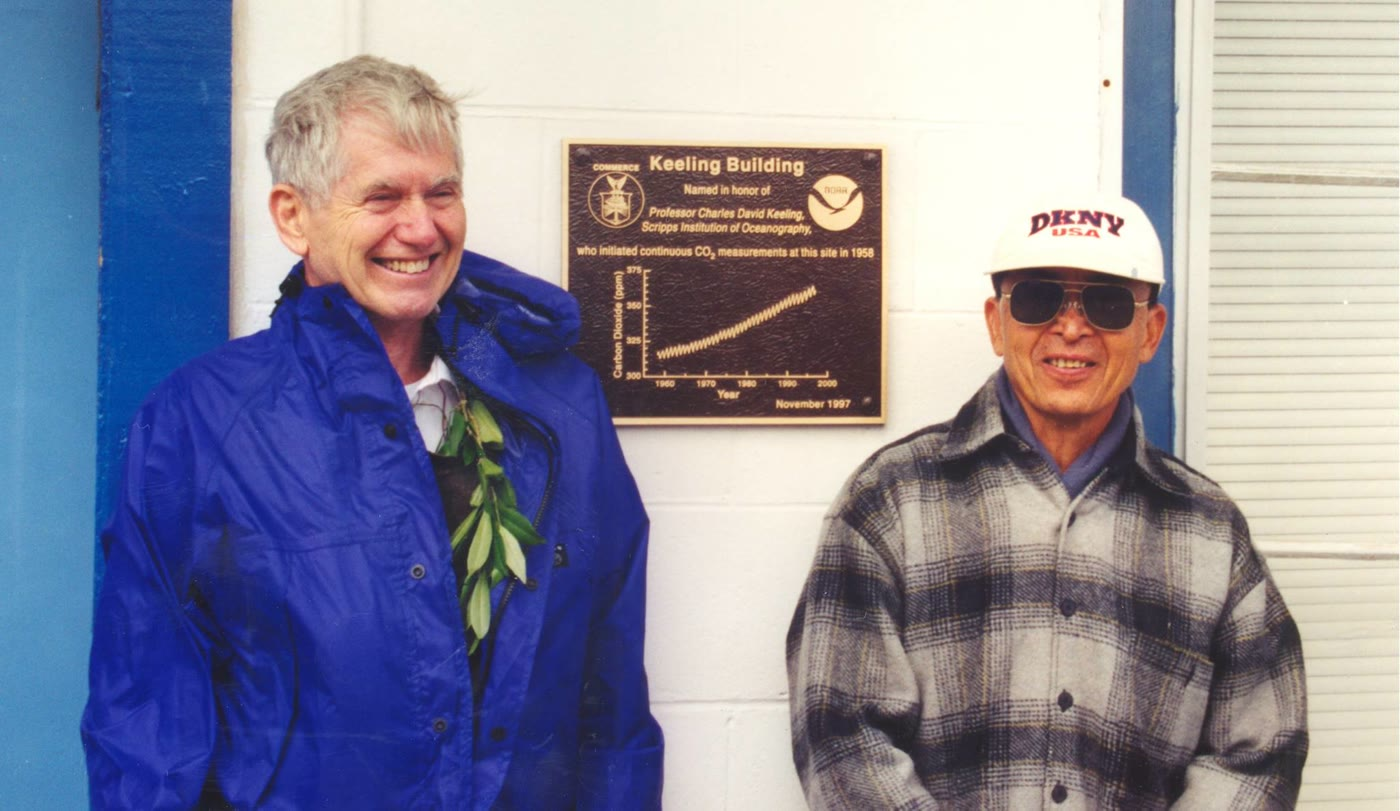
\includegraphics[width=0.62\linewidth]{images/book2/g12-noaa-keeling-chin-1997.jpg}

{\small تشارلز ديفيد كيلينغ (في اليسار) وجون تشين في مرصد ماونا لوا
عام 1997، بجانب اللوحة التي تسمّي مبنى باسم كيلينغ.
الصورة: جون ميلر، الإدارة الوطنية للمحيطات والغلاف الجوي الأمريكية (ملك عام).}
\end{center}
\end{history}

\section{تمارين}

\begin{exercise}[$\star$]\label{exo:g12:climate-change:1}
ما \omterm{def:g12:climate-change:forcing}{التأثير الإشعاعي} لتغيّر في النظام المناخي؟ وبأي
وحدة يُقاس، وماذا تعني إشارته؟
\end{exercise}

\begin{exercise}[$\star$]\label{exo:g12:climate-change:2}
في أي شهر من السنة يكون تركيز ثاني أكسيد الكربون في ماونا لوا
أعلى ما يكون، وفي أيها يكون أدنى ما يكون؟ فسّر التأرجح السنوي.
\end{exercise}

\begin{exercise}[$\star$]\label{exo:g12:climate-change:3}
بمفردات التقييمات، ما الاحتمال الذي تعنيه \emph{مرجح
جدًا}؟ وماذا تعني \emph{مرجح}؟ وماذا يعني مدى مكتوب
$[0.95 \text{, } 1.20]$؟
\end{exercise}

\begin{exercise}[$\star$]\label{exo:g12:climate-change:4}
من الطاقة الإضافية التي كسبها النظام المناخي في العقود الأخيرة،
ما الحصة التي ذهبت إلى المحيط؟ ولماذا يفسر هذا ارتفاع مستوى سطح البحر
حتى من دون ذوبان الجليد؟
\end{exercise}

\begin{exercise}[$\star$]\label{exo:g12:climate-change:5}
اذكر \omterm{def:g12:climate-change:feedback}{تغذيتين راجعتين} مناخيتين موجبتين، والاستجابة السالبة التي تحدّ من
الاحترار. واشرح كلًّا منها في جملة واحدة.
\end{exercise}

\begin{exercise}[$\star\star$]\label{exo:g12:climate-change:6}
كان المتوسط السنوي لتركيز ثاني أكسيد الكربون في ماونا لوا
\qty{315.98}{ppm} عام 1959 و\qty{427.35}{ppm} عام 2025. بكم جزءًا من المليون،
وبأي نسبة مئوية، ازداد؟ وما متوسط الزيادة في
السنة على امتداد الفترة كلها؟
\end{exercise}

\begin{exercise}[$\star\star$]\label{exo:g12:climate-change:7}
استعمل القانون اللوغاريتمي في الفصل، مع $F_{2\times} =
\qty{3.93}{W/m^2}$ و$C_0 = \qty{278}{ppm}$، لحساب \omterm{def:g12:climate-change:forcing}{تأثير}
ثاني أكسيد الكربون عند \qty{427.35}{ppm}، وهو المتوسط السنوي لعام 2025.
\end{exercise}

\begin{exercise}[$\star\star$]\label{exo:g12:climate-change:8}
بمعدل \qty{3.7}{mm} في السنة، وهو معدل 2006--2018، بكم كان مستوى البحر سيرتفع
في 30 سنة؟ وكم مرة يكون هذا المعدل أسرع من معدل
1901--1971، البالغ \qty{1.3}{mm} في السنة؟
\end{exercise}

\begin{exercise}[$\star\star$]\label{exo:g12:climate-change:9}
باستعمال $\Delta T = F/\lambda$ مع $\lambda = \qty{1.16}{W.m^{-2}.\degreeCelsius^{-1}}$،
احسب الاحترار عند التوازن الذي سيحدثه التأثير البشري الكلي لعام 2019،
\qty{2.72}{W/m^2}. والاحترار المرصود الذي سببه الإنسان لا يتجاوز
نحو \qty{1.07}{\degreeCelsius}. اذكر السبب الرئيسي للفرق.
\end{exercise}

\begin{exercise}[$\star\star$]\label{exo:g12:climate-change:10}
غيّرت الشمس والبراكين درجة الحرارة العالمية بين 1850--1900
و2010--2019 بمقدار $-0.1$ إلى $+\qty{0.1}{\degreeCelsius}$، في حين كان الاحترار
المرصود نحو \qty{1.06}{\degreeCelsius}. ماذا تستنتج؟ وأي
سبب طبيعي آخر يجب استبعاده أيضًا، وماذا يقول
التقييم عنه؟
\end{exercise}

\begin{exercise}[$\star\star$]\label{exo:g12:climate-change:11}
باستعمال جدول الإسقاطات، في أي \omterm{def:g12:climate-change:scenario}{السيناريوهات} يكون احترار
2081--2100 على نحو مرجح جدًا دون \qty{2}{\degreeCelsius}؟ وفي أيها يكون
على نحو مرجح جدًا فوق \qty{2}{\degreeCelsius}؟
\end{exercise}

\begin{exercise}[$\star\star\star$]\label{exo:g12:climate-change:12}
أحدث الهباء الجوي \omterm{def:g12:climate-change:forcing}{تأثيرًا} قدره نحو $-0.22$ و$\qty{-0.84}{W/m^2}$
(عبر ضوء الشمس وعبر السحب). لو أزيل كل الهباء الجوي من
الهواء وبقي كل شيء آخر كما كان عام 2019، فكم يصير التأثير البشري
الكلي؟ وبكم يزداد الاحترار عند التوازن، مع
$\lambda = \qty{1.16}{W.m^{-2}.\degreeCelsius^{-1}}$؟
\end{exercise}

\begin{exercise}[$\star\star\star$]\label{exo:g12:climate-change:13}
بيّن، انطلاقًا من القانون اللوغاريتمي، أن الانتقال من \qty{278}{ppm} إلى
\qty{556}{ppm} والانتقال من \qty{556}{ppm} إلى \qty{1112}{ppm} يضيفان \omterm{def:g12:climate-change:forcing}{التأثير}
نفسه. ما \omterm{def:g12:climate-change:forcing}{التأثير} الكلي عند \qty{1112}{ppm}؟
\end{exercise}

\begin{exercise}[$\star\star\star$]\label{exo:g12:climate-change:14}
اشتق القانون اللوغاريتمي بالنسبة إلى $C$. ما \omterm{def:g12:climate-change:forcing}{التأثير} الذي يضيفه
جزء إضافي واحد من المليون من ثاني أكسيد الكربون عند \qty{280}{ppm}، وما الذي يضيفه عند
\qty{420}{ppm}؟ علّق.
\end{exercise}

\begin{exercise}[$\star\star\star$]\label{exo:g12:climate-change:15}
من دون أي \omterm{def:g12:climate-change:feedback}{تغذية راجعة} سوى الإشعاع الإضافي إلى الفضاء،
$\lambda_0 = \qty{3.22}{W.m^{-2}.\degreeCelsius^{-1}}$. احسب الاحترار
لمضاعفة ثاني أكسيد الكربون ($F_{2\times} = \qty{3.93}{W/m^2}$) مع
$\lambda_0$، ثم مع $\lambda = \qty{1.16}{W.m^{-2}.\degreeCelsius^{-1}}$. بأي
عامل تضخّم \omterm{def:g12:climate-change:feedback}{التغذيات الراجعة} الاحترار؟
\end{exercise}

\section{مسألة: منحنى كيلينغ بالأرقام}

\begin{problem}[{مسألة نهاية الأسبوع --- من التنفس السنوي للغطاء
النباتي إلى السنة التي تُبلغ فيها المضاعفة}]
\label{pb:g12:climate-change:1}
% ledger: data:co2-mlo (annual means 1960 316.91, 1970 325.68, 2015 401.01,
% 2025 427.35; seasonal departures May +3.37, September -3.51, means of
% 2015-2024; all from figdata/grade-12/climate_records.py), noaa:mlo-site,
% ipcc:erf-2xco2, ipcc:ecs, ipcc:feedbacks, ipcc:co2-2myr
تنزّل طالبة سجل ماونا لوا وتعالجه في
جدول بيانات. ففي 2015--2024، يقع التركيز الشهري في المتوسط
أعلى من الاتجاه المنعَّم بمقدار \qty{3.37}{ppm} في مايو وأدنى منه بمقدار \qty{3.51}{ppm}
في سبتمبر. والمتوسطات السنوية \qty{316.91}{ppm} عام 1960،
و\qty{325.68}{ppm} عام 1970، و\qty{401.01}{ppm} عام 2015، و\qty{427.35}{ppm}
عام 2025. وكان تركيز عام 1750 \qty{278}{ppm}. استعمل القانون
اللوغاريتمي مع $F_{2\times} = \qty{3.93}{W/m^2}$.

\medskip
\noindent\textbf{الجزء الأول --- تنفس الغطاء النباتي.}
\begin{enumerate}
  \item ما سعة الدورة السنوية من القمة إلى القاع؟
  \item فسّر لماذا يكون التركيز أعلى ما يكون في مايو وأدنى ما يكون في
        سبتمبر.
  \item الدورة أضعف بكثير في هواء نصف الكرة الجنوبي.
        اقترح سببًا لذلك.
  \item لماذا بُني المرصد على ارتفاع \qty{3397}{m}، على بركان في
        وسط المحيط الهادئ؟
\end{enumerate}

\medskip
\noindent\textbf{الجزء الثاني --- الاتجاه.}
\begin{enumerate}[resume]
  \item احسب متوسط الزيادة، بالجزء من المليون في السنة، على مدى 1960--1970.
  \item احسبه على مدى 2015--2025.
  \item بأي عامل ازداد معدل الزيادة؟
  \item بأي نسبة مئوية ارتفع التركيز بين 1750
        و2025؟
  \item لا تُظهر \omterm{def:g12:past-climates:ice-core}{العينات الجليدية} أبدًا أكثر من نحو \qty{300}{ppm} على مدى
        \num{800000} السنة الأخيرة. بكم جزءًا من المليون تتجاوز قيمة 2025
        هذا الحد؟
\end{enumerate}

\medskip
\noindent\textbf{الجزء الثالث --- التأثير.}
\begin{enumerate}[resume]
  \item احسب \omterm{def:g12:climate-change:forcing}{تأثير} ثاني أكسيد الكربون عام 2025.
  \item احسبه عام 1960، ثم احسب زيادة \omterm{def:g12:climate-change:forcing}{التأثير} بين 1960
        و2025.
  \item أي تركيز يضيف \qty{1}{W/m^2} إلى \omterm{def:g12:climate-change:forcing}{تأثير} عام 2025؟
  \item بمعدل الزيادة في 2015--2025، كم سنة يستغرق ذلك؟
\end{enumerate}

\medskip
\noindent\textbf{الجزء الرابع --- المضاعفة.}
\begin{enumerate}[resume]
  \item ما التركيز الذي يمثل مضاعفة قيمة عام 1750؟ وأي
        \omterm{def:g12:climate-change:forcing}{تأثير} يحدثه؟
  \item بأفضل تقدير \omterm{def:g12:climate-change:ecs}{لحساسية المناخ عند التوازن}،
        ما الاحترار عند التوازن الذي يسببه؟ أعطِ المدى المرجح.
  \item ما معامل \omterm{def:g12:climate-change:feedback}{التغذية الراجعة} $\lambda$ الذي تقتضيه حساسية قدرها
        \qty{3}{\degreeCelsius}؟ قارنه بالقيمة
        \qty{1.16}{W.m^{-2}.\degreeCelsius^{-1}} التي نحصل عليها بجمع
        \omterm{def:g12:climate-change:feedback}{التغذيات الراجعة}.
  \item لماذا لا يبلغ السطح هذا الاحترار في اليوم الذي
        تُبلغ فيه المضاعفة؟
  \item لماذا يكون الحساب الذي يكتفي بمدّ معدل الزيادة الحالي \omterm{def:g12:climate-change:scenario}{سيناريو}،
        لا إسقاطًا من النوع الذي تقدمه التقييمات؟
  \item لو بقي معدل الزيادة في 2015--2025 على حاله، ففي أي سنة
        تُبلغ مضاعفة تركيز عام 1750؟
\end{enumerate}
\end{problem}
